\chapter{Recurrent Neural Networks}
% Authors: Qintai Liu
% Lecture date: 3/11/2019

% Editor: Michael Gold
% Last edited: 11/7/2019


\section{ High-Level Overview of Recurrent Neural Networks }

As Convolutional Neural Networks naturally lend themselves to images, Recurrent Neural Networks (RNNs),  including LSTMs and Transformers, lend themselves similarly to sequential data. These might take the form of time series, speech recognition, learning grammars (language translators, name generators, etcetera) or musical rhythms - among others. More precisely one can define them to be directed graphs mapping to a temporal sequence.\\

Visual captioning \cite{DBLP:journals/corr/VinyalsTBE16} is another interesting application, where they combine RNNs and CNNs in order to attempt to generate a text description of a scene \ref{fig:visual_caption}

\begin{figure}
    \centering
    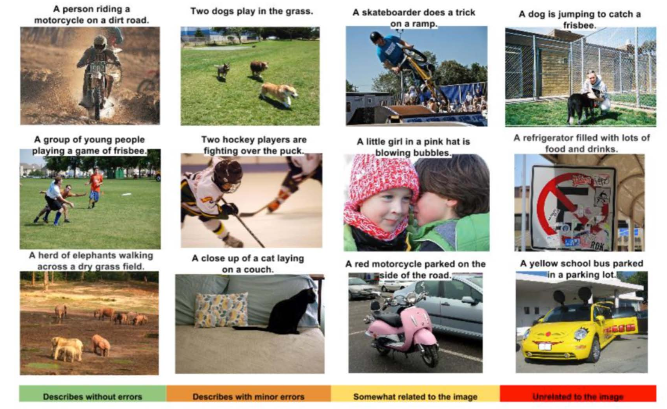
\includegraphics[width=\textwidth]{figs/image_captioning.png}
    \caption{Vinyals et al. (2016) Show \& Tell: Lessons Learned from the 2015 MSCOCO Image Captioning Challenge}
    \label{fig:visual_caption}
\end{figure}

\subsection{Simple Recurrent Net}
\label{sec:SimpleRecNet}
% Authors: Qintai Liu
% Lecture date: 3/11/2019

RNNs are designed to capture sequential information.
Some of the inputs of traditional neural network are independent of each other.
But in many tasks, the inputs are actually dependent on each other.
In order to predict what the next word is in a sentence, you must know which words appear before it.
Recurrent nets perform the same task for every element of a sequence, with the output being depended on the previous computations. 
RNNs can take advantage of information in arbitrarily long sequences theoretically, but in reality they are limited to capturing long-term dependencies.

\begin{figure}[h]
    \centering
    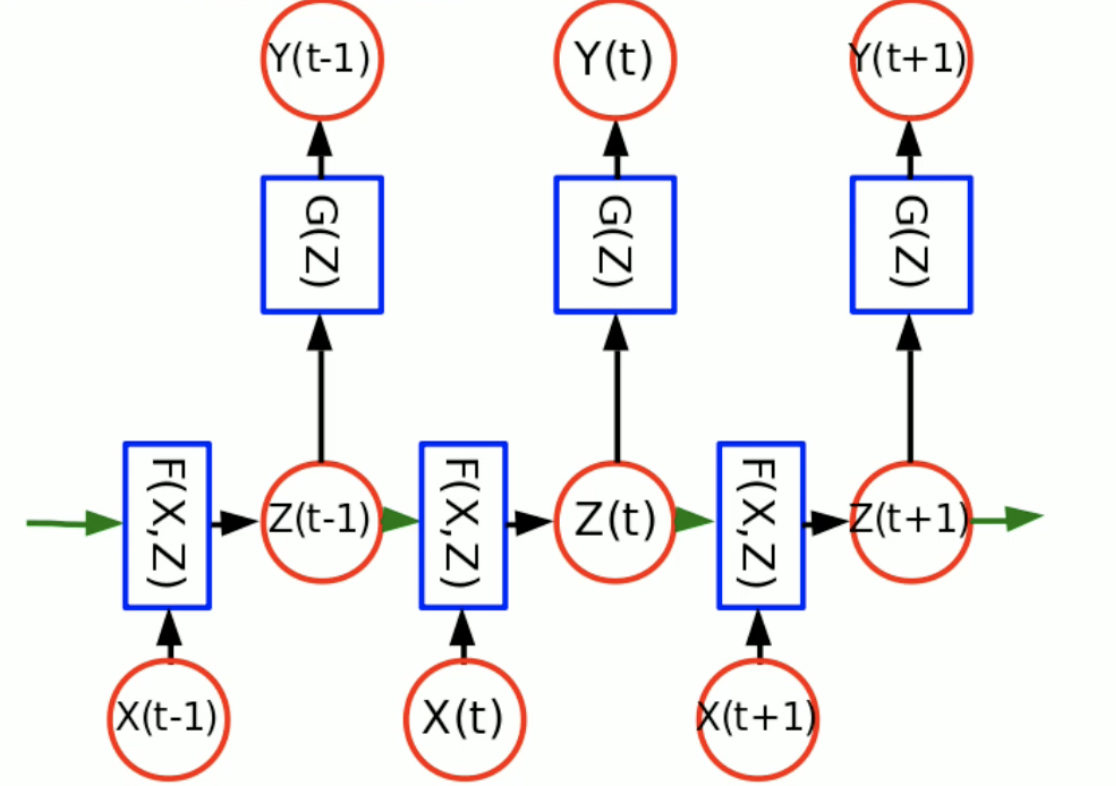
\includegraphics[width=150pt]{figs/rnn.png}
    \caption{Simple Recurrent Net}
    \label{fig:Simple RNN}
\end{figure}

\begin{itemize}
  \item $\vect{x_{t}}$ is the input at time step $t$
  \item $\vect{z_{t}}$ is the hidden state at time $t$. $\vect{z_{t}}$ is calculated based on the input at the current step and the previous hidden state:
  $\vect{z_t} = F(\vect{x_t}, \vect{z_{t-1}})$
  \item $\vect{y_t}$ is the output at step $t$. $\vect{y_t} = G(\vect{z_t})$
\end{itemize}




\subsection{Sequence to vector}
Explanation: input: a sequence of words; output: a scalar value or a vector (see Figure \ref{fig:seq_to_vec}).\\
\begin{figure}[ht]
    \centering
    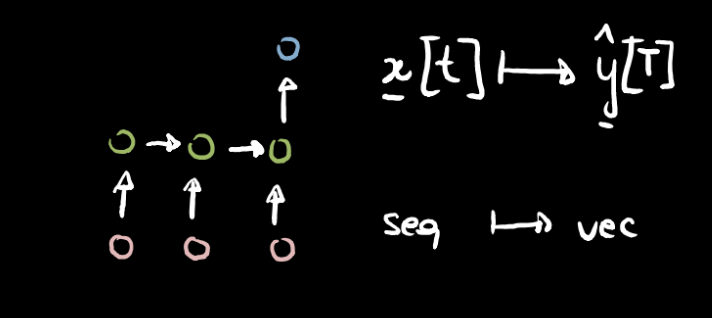
\includegraphics[width=200pt]{figs/seq_to_vec.png}
    \caption{A hand-drawn diagram showing the sequence to vector rationale in the neural networks. Red, green, blue circles are input,hidden,output nodes, respectively. A sequence of inputs are given to the network and there is only one output in the end.}
    \label{fig:seq_to_vec}
\end{figure}
\\
Example: learning to execute (Zaremba \& Sutskever, 2015)\\
Neural network is trained to interpret several lines of python codes and report the result of the running code (see Figure \ref{fig:learning_to_execute}). \\
\begin{figure}[ht]
    \centering
    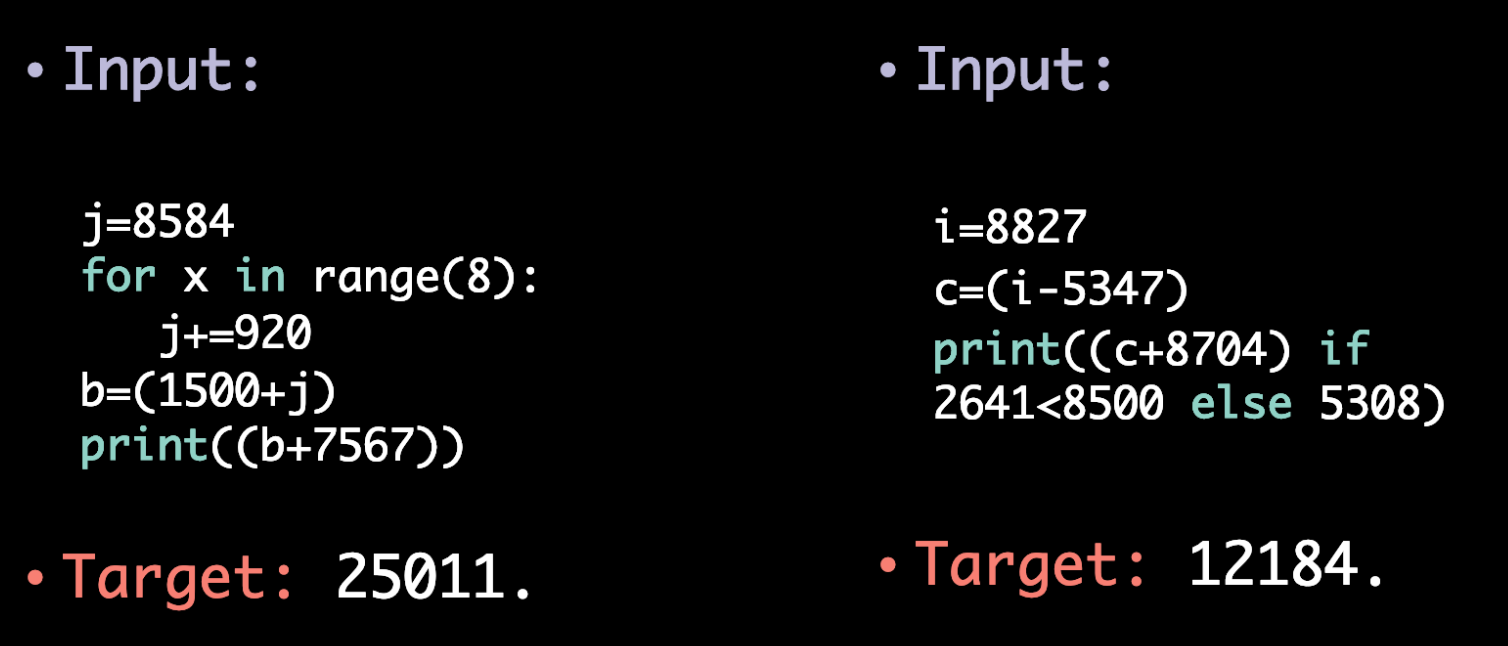
\includegraphics[width=200pt]{figs/learning_to_execute.png}
    \caption{An example of sequence to vector rationale. A paragraph of Python code is given to the network as an input and the execution output of the Python code is supposed to be the output of the network.}
    \label{fig:learning_to_execute}
\end{figure}

\subsection{Sequence to vector to sequence}
Explanation: a sequence of words $\rightarrow$ hidden representations(vector) $\rightarrow$ output sequence (see Figure \ref{fig:seq_to_vec_to_seq}).\\
\begin{figure}[ht]
    \centering
    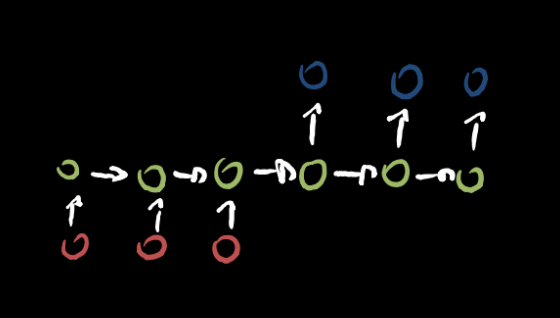
\includegraphics[width=200pt]{figs/seq_to_vec_to_seq.png}
    \caption{A hand-drawn diagram showing the sequence to vector to sequence rationale in the neural networks. Red, green, blue circles are input,hidden,output nodes, respectively. A sequence of inputs are given to the network and used to compute hidden state. Hidden state variable are  then used to generate a sequence of outputs. }
    \label{fig:seq_to_vec_to_seq}
\end{figure}
\\
Example: phrase representation clustering (Cho et al., 2014)\\
Semantically close phrases are close to each other on the representation map (Figure \ref{fig:phrase_representaion})\\
\begin{figure}[ht]
    \centering
    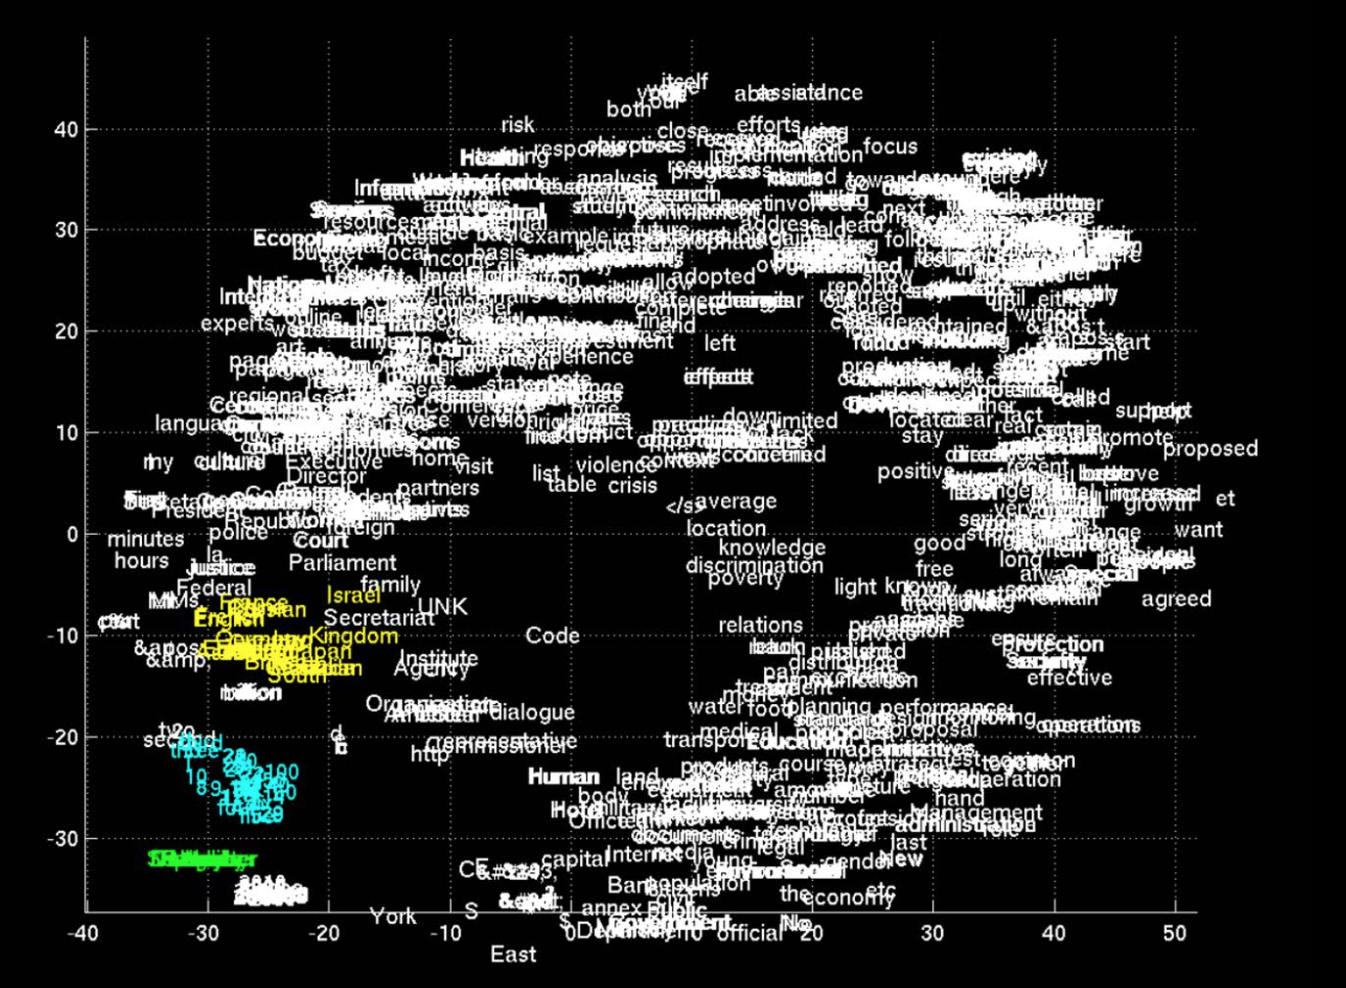
\includegraphics[width=200pt]{figs/phrase_representation.png}
    \caption{An example of sequence to vector to sequence rationale. Words are clustered according to their semantics}
    \label{fig:phrase_representaion}
\end{figure}
One interesting characteristic is one could perform arithmetic calculation of the semantics in hidden variable space. For example, we have\\
\begin{equation*}
    h('king')-h('men')+h('women')=h('queen')
\end{equation*}
where h(X) is the hidden state of word 'X'. \\

\subsection{Sequence to sequence}
Explanation: a sequence of words $\rightarrow$ another sequence of words (see Figure \ref{fig:seq_to_seq}).\\
\begin{figure}[ht]
    \centering
    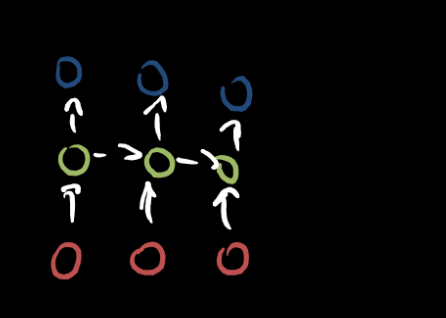
\includegraphics[width=200pt]{figs/seq_to_seq.png}
    \caption{A hand-drawn diagram showing the sequence to sequence rationale in the neural networks. Red, green, blue circles are input, hidden, output nodes, respectively. A sequence of inputs are given to the network and used to compute hidden state. Hidden state variable are used to generate a sequence of outputs in real time.}
    \label{fig:seq_to_seq}
\end{figure}
\\
Example: auto completion: Once a character is typed, there will be a new sequence of suggestions of auto completion. \\
\\
Example: RNN writer(Sloan(2016))\\
Neural network is trained on sci-fi novels and could be used to auto complete the sci-fi novel.\\
Visit \href{github.com/robinsloan/rnn-writer}{github.com/robinsloan/rnn-writer} for more details.\\





\section{Issue of Simple Recurrent Net}
% Authors: Qintai Liu
% Lecture date: 3/11/2019
\subsection{Backpropagation Through Time}
% Authors: Qintai Liu
% Lecture date: 3/11/2019
In order to know the issue of simple RNN, we first need to know how the gradient is calculated in terms of RNN. Suppose the hidden state($\vect{z_t}$) is calculated as below:

\[\vect{\bar{z_t}} = \matr{W_X} \vect{x_t} + \matr{W_Z} \vect{z_{t-1}}\]
\[\vect{z_t} = f(\bar{\vect{z_t}})\]
\[\vect{y_t} = g(\vect{z_t})\]

To measures the effect of the $(t-n)$-th input symbot $x_{t-n}$, where $n\leq{t}$, on the $t$-th hidden state $\vect{z_t}$ of the simple recurrent neural network, we need to calculate the derivative shown below
\[\frac{\partial \vect{z_t}}{\partial \vect{x_{t-n}}}=\frac{\partial \vect{z_t}}{\partial \vect{z_{t-n}}}\frac{\partial \vect{z_{t-n}}}{\partial \vect{\bar{z}_{t-n}}}\frac{\partial \vect{\bar{z}_{t-n}}}{\partial \vect{x_{t-n}}}\]

Among these three terms in the right hand side of the above equation, we will focus on the first term

\begin{equation} \label{eq:bptt}
\frac{\partial \vect{z_t}}{\partial \vect{z_{t-n}}} = (\underbrace{\frac{\partial \vect{z_t}}{\partial \vect{\bar{z}_{t}}}}_{a}\underbrace{\frac{\partial \vect{\bar{z}_{t}}}{\partial \vect{z_{t-1}}}}_{b})
(\underbrace{\frac{\partial \vect{z_{t-1}}}{\partial \vect{\bar{z}_{t-1}}}}_{a}\underbrace{\frac{\partial \vect{\bar{z}_{t-1}}}{\partial \vect{z_{t-2}}}}_{b}) \ldots 
(\underbrace{\frac{\partial \vect{z_{t-n+1}}}{\partial \vect{\bar{z}_{t-n+1}}}}_{a}\underbrace{\frac{\partial \vect{\bar{z}_{t-n+1}}}{\partial \vect{z_{t-n}}}}_{b})
\end{equation}

First, consider \cref{eq:bptt}(a), which is the derivative of a nonlinear activation function used in the simple recurrent neural network.

Next, we look at \cref{eq:bptt}(b). We know

\[\frac{\partial \vect{\bar{z}_{t}}}{\partial \vect{z_{t-1}}} = \matr{W_Z}\]

From these two, we get
\begin{align} \label{eq:bptt_result}
\begin{split}
\frac{\partial \vect{z_t}}{\partial \vect{z_{t-n}}} &= (\frac{\partial \vect{z_t}}{\partial \vect{\bar{z}_{t}}}\frac{\partial \vect{\bar{z}_{t}}}{\partial \vect{z_{t-1}}})
(\frac{\partial \vect{z_{t-1}}}{\partial \vect{\bar{z}_{t-1}}}\frac{\partial \vect{\bar{z}_{t-1}}}{\partial \vect{z_{t-2}}}) \ldots 
(\frac{\partial \vect{z_{t-n+1}}}{\partial \vect{\bar{z}_{t-n+1}}}\frac{\partial \vect{\bar{z}_{t-n+1}}}{\partial \vect{z_{t-n}}}) \\
&= (\frac{\partial \vect{z_t}}{\partial \vect{\bar{z}_{t}}}\matr{W_Z})
(\frac{\partial \vect{z_{t-1}}}{\partial \vect{\bar{z}_{t-1}}}\matr{W_Z}) \ldots 
(\frac{\partial \vect{z_{t-n+1}}}{\partial \vect{\bar{z}_{t-n+1}}}\matr{W_Z}) \\
&= \prod\limits_{i=t-n+1}^{t} (\frac{\partial \vect{z_i}}{\partial \vect{\bar{z}_{i}}}\matr{W_Z})
\end{split}
\end{align}

Suppose the recurrent activation function $f$ is linear, \cref{eq:bptt_result} is reduced to
\begin{equation} \label{eq:bptt_linear_result}
\frac{\partial \vect{z_t}}{\partial \vect{z_{t-n}}} = \matr{W_Z}^{n-1}
\end{equation}


\subsection{Exploding Gradients}
% Authors: Qintai Liu
% Lecture date: 3/11/2019
When we do back-propagation in the recurrent neural networks, gradients of loss with respect to the weights can accumulate and result in very large gradients.
These in turn cause large updates to the neural network weights.

% In recurrent neural networks, gradients can accumulate during an update and result in very large gradients. 
% These in turn result in large updates to the network weights, and in turn, an unstable network. 

The explosion occurs through exponential growth by repeatedly multiplying gradients through the network layers that have values larger than $1.0$.

From \cref{eq:bptt_linear_result}, $\frac{\partial \vect{z_t}}{\partial \vect{z_{t-n}}}$ will likely explode as $n \rightarrow \inf$ if $e_{max} > 1$, where $e_{max}$ is the largest eigenvalue of $\matr{W_Z}$.

\subsection{Vanishing Gradients}
% Authors: Qintai Liu
% Lecture date: 3/11/2019
In recurrent neural networks, the gradients of loss with respect to the weights may also get smaller and smaller as we keep on moving backward in the network. 
In other words, the weights in the earlier layers get updated slowly compared with the neurons in the later layers.
These in turn result in a difficulty for training earlier layers of recurrent neural networks.

From \cref{eq:bptt_linear_result}, $\norm{\frac{\partial \vect{z_t}}{\partial \vect{z_{t-n}}}} \rightarrow 0$ when $e_{max} < 1$, where $e_{max}$ is the largest eigenvalue of $\matr{W_Z}$.

\section{Gradient clipping}
% Authors: Qintai Liu
% Lecture date: 3/11/2019
Fortunately it's easy to solve the problem of exploding gradients by doing gradient clipping \cite{1211.5063}.
First, in order to detect whether the exploding gradient arises, we could inspect the norm of the gradient of loss with respect to the parameters $\norm{\nabla}$.
If the gradient's norm is larger than some predefined threshold $\tau > 0$, we can renormalize the norm of the gradient to be $\tau$.

\[
\widetilde{\nabla}=\left\{
            \begin{array}{ll}
              \tau\frac{\nabla}{\norm{\nabla}} & \text{if}  \norm{\nabla}>\tau\\
              \nabla & \text{otherwise}
            \end{array}
          \right.
\]

\section{Long Short-Term Memory}
\label{sec:long-short-term-memory}
% Authors: Qintai Liu
% Lecture date: 3/11/2019


\begin{figure}[h]
  \centering
      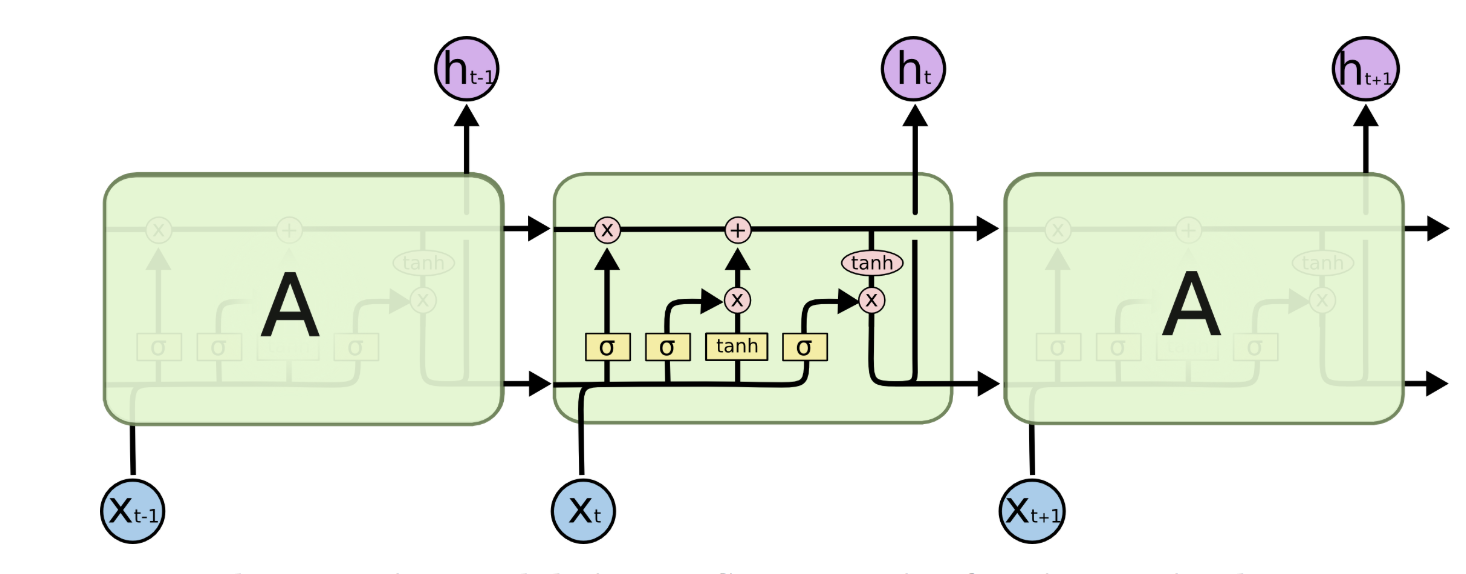
\includegraphics[width=0.8\textwidth,height=4.5cm]{figs/lstm.png}
          \caption{
            The repeating module in an LSTM contains four interacting layers.
            \href{http://colah.github.io/posts/2015-08-Understanding-LSTMs/}{Source}
          }
          \label{fig:lstm}
\end{figure}

Long Short Term Memory networks \cite{article-lstm} are a special kind of RNN, capable of learning long-term dependencies. 
They work tremendously well on a large variety of problems, and are now widely used.
LSTMs are explicitly designed to avoid the long-term dependency problem. 
Below is how LSTM works

The forget gate in LSTM is to decide what information we’re going to throw away from the cell state.
\[\vect{f_t} = \sigma(\matr{W_{fh}}\vect{h_{t-1}}+\matr{W_{fx}}\vect{x_t} + \vect{b_f}) \]

Input gate decides which values we’ll update
\[\vect{i_t} = \sigma(\matr{W_{ih}}\vect{h_{t-1}} + \matr{W_{ix}}\vect{x_t} + \vect{b_i})\]

New candidate cell state is to decide what new information we’re going to store in the cell state.
\[\vect{\widetilde{c}_t} = tanh(\matr{W_{ch}}\vect{h_{t-1}} + \matr{W_{cx}}\vect{x_t} + \vect{b_c})\]

New cell state:
\[\vect{c_t} = \vect{f_t}*\vect{c_{t-1}} + \vect{i_t}*\vect{\widetilde{c}_t}\]

Output Gate decides what parts of the cell state we’re going to output.
\[\vect{o_t} = \sigma(\matr{W_{oh}}\vect{h_{t-1}} + \matr{W_{ox}}\vect{x_t} + \vect{b_o})\]

Output:
\[\vect{h_t} = \vect{o_t}*tanh\vect{(c_t)}\]

\section{Gated Recurrent Units}
% Authors: Qintai Liu
% Lecture date: 3/11/2019

\begin{figure}[h]
  \centering
      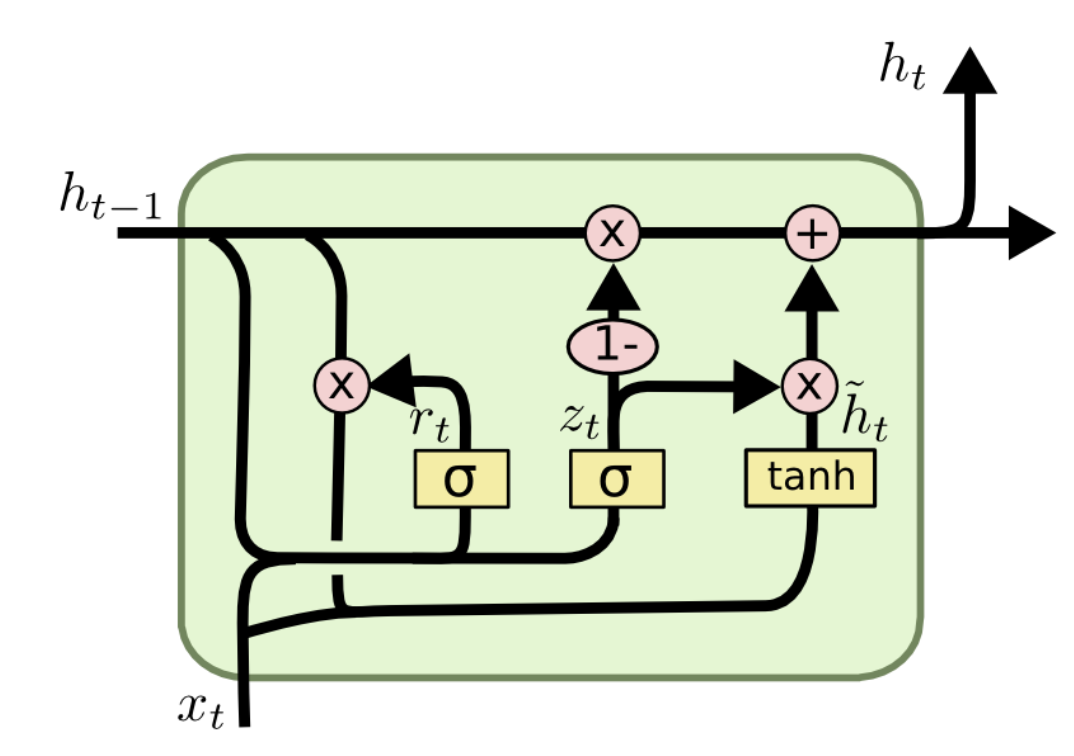
\includegraphics[width=0.5\textwidth,height=4.5cm]{figs/GRU.png}
          \caption{
            Gated Recurrent Units
            \href{http://colah.github.io/posts/2015-08-Understanding-LSTMs/}{Source}
          }
          \label{fig:gru}
\end{figure}

A slightly more dramatic variation on the LSTM is the Gated Recurrent Unit \cite{1406.1078}.
It combines the forget and input gates into a single “update gate.” 
It also merges the cell state and hidden state, and makes some other changes. 
The resulting model is simpler than standard LSTM models.
Below is how GRU works

The update gate decides what information from the past would be passed to the next cell state.

\[\vect{z_t} = \sigma(\matr{W_{zh}}\vect{h_{t-1}}+\matr{W_{zx}}\vect{x_t} + \vect{b_z}) \]

The reset gate determine what information would be discarded from previous cell states.

\[\vect{r_t} = \sigma(\matr{W_{rh}}\vect{h_{t-1}}+\matr{W_{rx}}\vect{x_t} + \vect{b_r}) \]

Then the current memory content update the stories the latest important information by using the reset gate.

\[\vect{\widetilde{h}_t} = \tanh(\matr{W_{hr}}(\vect{r_t}*\vect{h_{t-1}}) + \matr{W_{hx}}\vect{x_t} + \vect{b_h})\]

Finally, the final cell state updates the information gained from the current unit and passed it to the next cell.

\[\vect{h_t} = (1-\vect{z_t})*\vect{h_{t-1}} + \vect{z_t}*\vect{\widetilde{h}_t}\]

% Authors: Benjamin Ahlbrand (editor), Xingyu Ding, Haoran Anthony Su, 3/12/19.


\section{RNN training}
\subsection{BPTT: backpropagation through time}
\begin{figure}[ht]
    \centering
    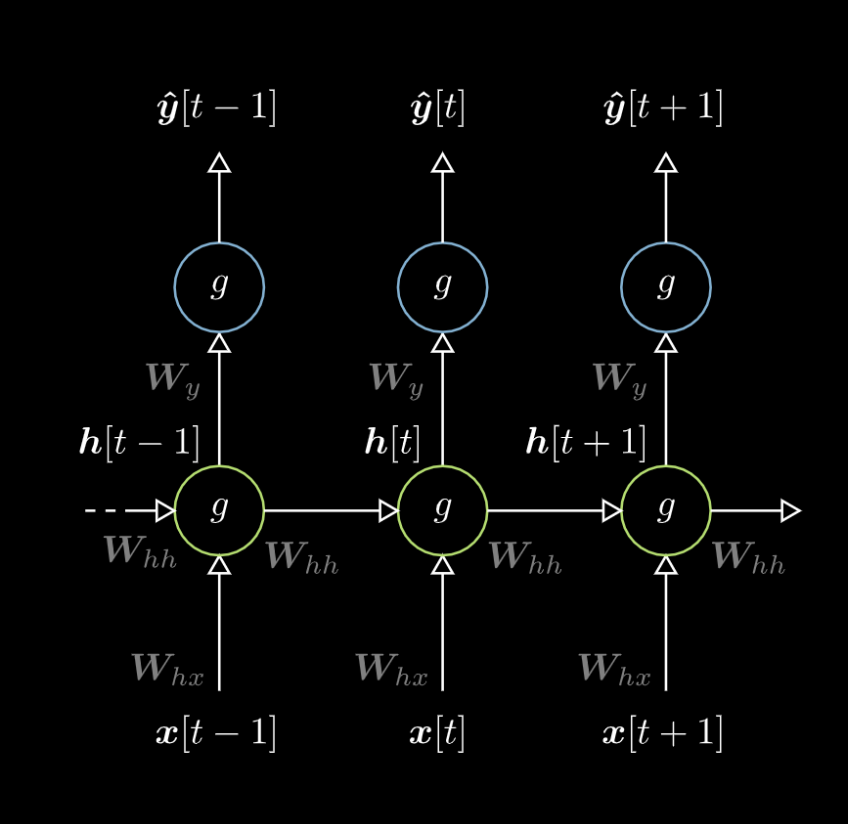
\includegraphics[width=200pt]{figs/bptt.png}
    \caption{A diagram showing how the values are propagated in a RNN. At each time point t, y is calculated using h from the previous time step and current x.  g() is the transfer function, ReLu for example. h[t] is the value of hidden layer at time t. The initial state of h[t] is 0.}
    \label{fig:bptt}
\end{figure}
In order to train a RNN, we are supposed to use backpropagation through time(BPTT) (see Figure \ref{fig:bptt}). In order to calculate the hidden state value h[t], we have\\
\begin{equation}
h[t] = g(W_{hx}x[t]+W_{hh}h[t-1]+b_h)
\end{equation}
To simplify the equation, we define $W_h$ as
\begin{equation}
    W_h = \begin{bmatrix}W_{hx} & W_{hh}\end{bmatrix}
\end{equation}
Thus, we could rewrite equation 1 as 
\begin{equation}
    h[t] = g(W_h\begin{bmatrix}x[t]\\h[t-1]\end{bmatrix} + b_h)
\end{equation}
$\hat{y}[t]$ could be calculated as shown in figure.\ref{fig:bptt_formula} and then we could use normal backpropagation algorithm except that we sum up the gradients at each time step.  
\begin{figure}[ht]
    \centering
    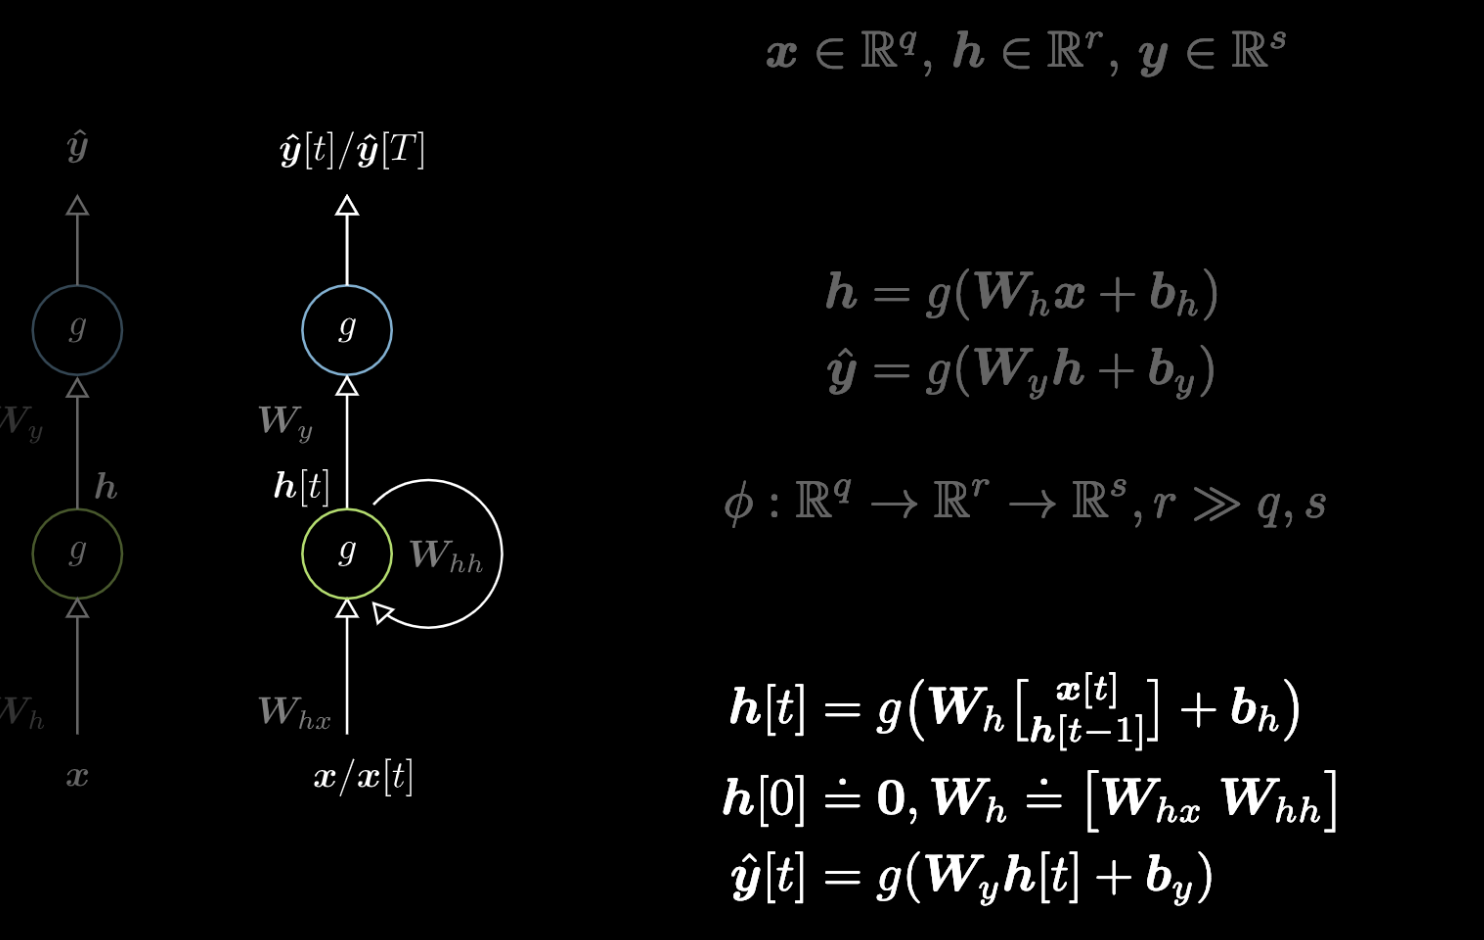
\includegraphics[width=200pt]{figs/bptt_formula.png}
    \caption{$\hat{y}[t]$ shares the same formula as traditional feedforward network. All we have to do is to use the chain rule and backpropagate the error to previous time step.}
    \label{fig:bptt_formula}
\end{figure}


\section{Batch-ification}
When dealing with text sample with large size, we could slice the text into different batches. For example, the batch-ification process for the following sequence of words should exhibit:\\
\begin{align*}
\begin{bmatrix}
    a & g & m & s\\
    b & h & n & t\\
    c & i & o & u\\
    d & j & p & v\\
    e & k & q & w\\
    f & l & r & x\\
\end{bmatrix}
\end{align*}
In this sequence of words, the batch size is 4. We then determine the input and output for our recurrent neural network, namely:\\
\begin{align*}
X[1:T] & = \begin{bmatrix}
        a & g & m & s\\
        b & h & n & t\\
        c & i & o & u\\
\end{bmatrix}
\end{align*}
\begin{align*}
Y[1:T] & = \begin{bmatrix}
        b & h & n & t\\
        c & i & o & u\\
        d & j & p & v\\
\end{bmatrix}
\end{align*}
Notice here $T = 3$ as we proceed three sequence of words. The next step is to perform back-propagation through time on the sequences of words, which is to say we calculate gradient descent horizontally and vertically. Every time we extract one word from the input sequence and we are aiming to predict the corresponding output in the output sequence. For example, when we select $X[1] = [a, g, m, s]$ as input, we train through the RNN to predict $Y[1] = [b, h, n, t]$. At the same time, we send the hidden representation h[1] forward to perform the RNN given $X[2]$ predicting $Y[2]$. After sending the final hidden representation $h[T-1]$ for the final set of $X[T]$ and $Y[T]$, we cut the gradient and conclude the temporal bulk of this batch. \\

The reason behind concluding the temporal bulk after we sending the last hidden representation of the RNN is that we need to stop the gradient descent eventually. Thus, the gradient descent from the following sequences of words is zero.(The PyTorch Auto-grad will handle this critical point.) Similarly, we also don't have the gradient coming from the past sequences before this batch.

\section{Vanishing of the Gradient and GRU}
The limitation of a recurrent Neural Network is the diminishing of the gradient back in time. A very strong gradient would be weakening back through time because of the way we initialize the weight-by selecting very small eigenvalues across zero. A powerful technique that preventing the gradient from vanishing back through time is by employing Gated Recurrent Unit (GRU).\\

GRU uses two gates-update gates and reset gates. A update gate helps the model to determine how information/gradient from the previous time steps need to pass along to the future. A reset gate, on the other hand, determine how much past information/gradient to forget. 

\section{Long Short Term Memory}
Long Short Term Memory, or typically referred to as LSTMs - these are second order RNNs, tend to imbue a sense of locality (spatial, temporal) to the network models.\\

The forward propagation of the RNN are represented by:\\
\begin{align*}
    h[t] & = g(W_{h} \begin{bmatrix}
        x[t] \\
        h[t - 1] \\
    \end{bmatrix}) + b_{h}\\
    \bar{y}[t] & = g(W_{y}h[t] + b_{y})
\end{align*}
The decomposition of a Gated Recurrent Unit (GRU) will be visualized as:\\
\begin{align*}
i[t] & = \sigma(W_{i} \begin{bmatrix} x[t] \\ h[t - 1] \\ \end{bmatrix}) + b_{i}\\
f[t] & = \sigma(W_{f} \begin{bmatrix} x[t] \\ h[t - 1] \\ \end{bmatrix}) + b_{f}\\ 
o[t] & = \sigma(W_{o} \begin{bmatrix} x[t] \\ h[t - 1] \\ \end{bmatrix}) + b_{o}\\
\bar{c}[t] & = \tanh(W_{c} \begin{bmatrix} x[t] \\ h[t - 1] \\ \end{bmatrix}) + b_{c}\\
c[t] & = f[t] \odot c[t-1] + i[t] \odot \bar{c}[t]\\
h[t] & = o[t] \odot \tanh(c[t])\\
\end{align*}
To control the output, take saturated (squashing / squeezing inputs to a range) sigmoid as an example which we could make the switch simply as 1 or 0, we could determine the hidden representation to be zero by setting the sigmoid function to be null; On the other hand, we could output accordingly by setting the sigmoid function to be 1.\\

To control the memory, we could manipulate the input network and the "don't forget" gate. Simply setting them both to zero, we could reset the memory. To keep the memory, we set the input unit to be zero and memory to be one using the sigmoid function to keep the memory without adding anything from the current input. Finally, we could write to the memory by setting the saturated sigmoid function both to be one to add input to the memory.\\

\section{ Transformers? Pay Attention! }
A new architecture has found popularity in many applications typically dominated by RNNs and LSTMs, Transformers - introduced by \cite{DBLP:journals/corr/VaswaniSPUJGKP17}. Transformers essentially add attention 
RNNs and LSTMs suffer issues with the memory bandwidth bound computations in training, where given the orthogonality of traditional convolutional networks to the GPU hardware, CNNs map perfectly to GPUs. Contrarily these hierachical (sometimes) sequential representations don't typically map quite so easily, and hence, performance suffers as a result.\\



\section{Why Is RNN Useful, And What Are The Drawbacks?}
%Authors: Sarthak Agarwal, Raghav Jajodia, Ieshan Vaidya
%2019-03-31

In lab8 we saw that RNN is useful to learn dependencies over time, and hence can model time dependent sequences effectively.
This means RNN can store context/history at any given time t, which can be used along with the input to predict the output. 
More details about RNN can be found in \hyperref[sec:SimpleRecNet]{Section 13.1}.


However, practically we observe that as the sequence length grows over time, RNN is not able to learn long term dependencies.
This is because of the \textbf{vanishing/exploding gradient} during \textbf{back-propagation through time}.
Back-propagation through time is the method of calculating gradients by unfolding the network in time and then applying normal back-propagation to the unfolded network.
If the the length of input sequence is large, then network is unfolded many number of times.
The consequence of this is that during back-propagation, gradient is multiplied many times (more the sequence length, more the number of multiplications). 


This causes the, gradient to either explode or vanish, which is undesirable.
To solve the issue of exploding gradient, we generally "clip" the gradient to avoid growing it bigger than a threshold value.
However RNN performs poorly for large length sequences because of vanishing gradient problem.

\section{Why Is LSTM Useful?}
%Authors: Sarthak Agarwal, Raghav Jajodia, Ieshan Vaidya
%2019-03-31
Vanishing gradient problem can be solved efficiently by using LSTMs.
LSTM stands for Long Short term Memory and it has been proven effective to model long term dependencies more effectively than RNN, meaning that LSTM has greater memory than RNN.
The reason for this is that LSTMs maintain a cell state which runs straight down the entire chain, with only some minor linear interactions.
They have the ability to either add or remove information to this cell state using gates namely the forget, input  and output gates.
More details about LSTM can be found \hyperref[sec:long-short-term-memory]{here}


The reason why vanishing gradient is handled better in case of LSTM is that gradient flows back effectively through the network because of the presence of relevant gates which makes it very easy for information to just flow along the cell state unchanged.


\section{Lab 8 - Result Analysis}
%Authors: Sarthak Agarwal, Raghav Jajodia, Ieshan Vaidya
%2019-03-31
In lab8, we try to classify a sequence of characters into categories Q,R,S,U. 
This classification is done on the basis of two characters X,Y which can be present anywhere in the sequence. 
In this experiment we compare the ability of RNN and LSTM to learn dependencies for different sequence lengths. The Difficulty and configurations of the experiment is explained in detail in \cref{sec:SeqClassification}. Here is the table of the test accuracies - 

\begin{center}
\begin{tabular}{ | p{3cm} | p{2cm} | p{2cm} | p{2cm} | p{2cm} | }
 \hline
   \textbf{DIFFICULTY} & \textbf{RNN (10 epochs)} & \textbf{LSTM (10 epochs)} & \textbf{RNN (100 epochs)} & \textbf{LSTM (100 epochs)} \\ 
 \hline
 \textbf{Easy} & 60.58\% & 79.33\% & 87.30\% & 87.50\% \\
 \hline
\textbf{Normal} & 24\% & 26\% & 71\% & 85\% \\ 
 \hline
 \textbf{Moderate} & 24.60\% & 28.43\% & 26.65\% & 84.37\% \\ 
 \hline
 \textbf{Hard} & 23.19\% & 25.10\% & 24.70\% & 25.30\% \\ 
 \hline
\end{tabular}

\end{center}
As we can see that LSTM outperforms RNN in almost all the cases.
We also observe that RNN and LSTM are not able to learn the sequence when ran for 10 epochs in case of MODERATE, NORMAL and HARD LEVEL.
When ran for 100 epochs, RNN and LSTM are not able to learn for HARD level, whereas they are able to learn other configurations. 